\section{Results}\label{sec:results}
We compare the greedy rule with uniform and random sampling on 200 synthetic
maps. Table~\ref{tab:results} lists the mean error after $n$ probes and the
mean run time; Figure~\ref{fig:error} shows the error curves.

\begin{table}[h]
\centering
\begin{tabular}{lcccccccc}
\toprule
Sampling scheme & $n=16$ & $n=32$ & $n=64$ & $n=128$ & $n=256$ & $n=512$ & Mean run time (ms) & Peak memory use (MB) \\
\midrule
Uniform grid sampling & 0.412 & 0.301 & 0.207 & 0.144 & 0.101 & 0.071 & 1.20 & 12.4 \\
Random (Poisson disk) sampling & 0.398 & 0.287 & 0.199 & 0.139 & 0.097 & 0.069 & 1.31 & 12.9 \\
Greedy adaptive rule (ours) & 0.351 & 0.192 & 0.088 & 0.031 & 0.011 & 0.004 & 3.84 & 14.1 \\
\bottomrule
\end{tabular}
\caption{Mean reconstruction error and cost over 200 maps.}
\label{tab:results}
\end{table}

\begin{figure}[h]
\centering
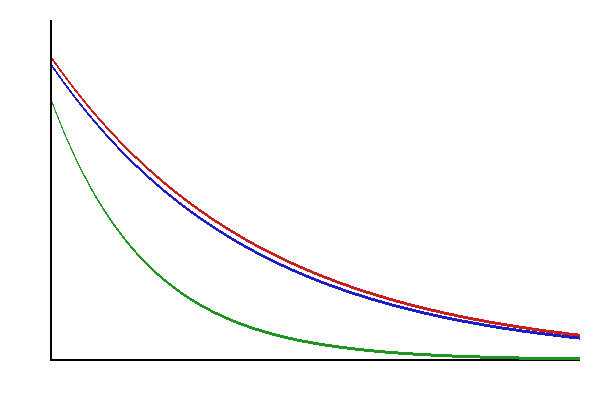
\includegraphics[width=1.25\textwidth]{figures/error}
\caption{Reconstruction error against the number of probes.}
\label{fig:erorr}
\end{figure}

The greedy rule overtakes both baselines after 32 probes and is an order of
magnitude more accurate at 256 probes, at roughly three times the run time.
Its advantage grows with sparsity, as the bound of Section~\ref{sec:bound}
predicts.
